%! Tex program = xelatex
\documentclass{article}
\usepackage[UTF8]{ctex}
\usepackage{tikz}
\begin{document}
  \begin{figure}
    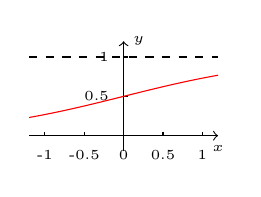
\begin{tikzpicture}
      \draw[->](-1.2,0)--(1.2,0)node[left,below,font=\tiny]{$x$};
      \draw[->](0,-0.2)--(0,1.2)node[right,font=\tiny]{$y$};
      \draw[dashed](-1.2,1)--(1.2,1);
      \foreach \x in {-1,-0.5,0,0.5,1}{\draw(\x,0)--(\x,0.05)node[below,outer sep=2pt,font=\tiny]at(\x,0){\x};}
      \foreach \y in {0.5,1}{\draw(0,\y)--(0.05,\y)node[left,outer sep=2pt,font=\tiny]at(0,\y){\y};}
      \draw[color=red ,domain=-1.2:1.2]plot(\x,{1/(1+(e^(-1*(\x))))});
    \end{tikzpicture}
  \end{figure}
该图的表达式是:
\[
sigmoid(x) = \frac{1}{1 + e^{-x}}
\]
\end{document}
